\chapter{Casi d'Uso}
\section*{Inizializzazione sistema}

\begin{figure}[ht]
  \centering
  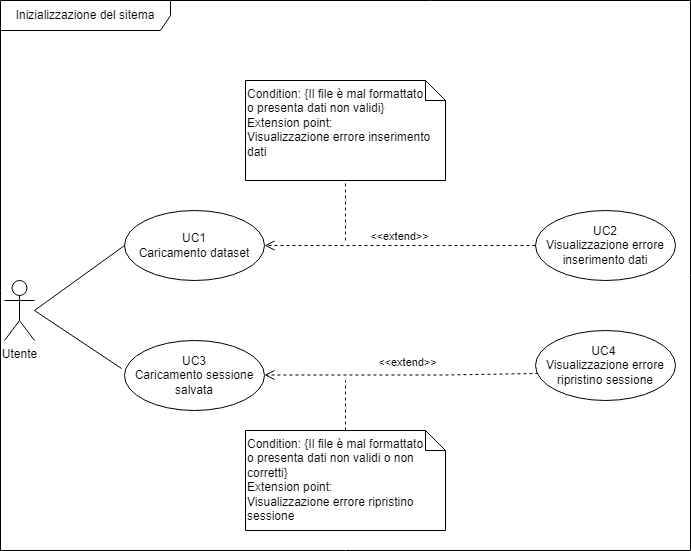
\includegraphics[width=\textwidth]{Iniz_sistema}
  \caption{Inizializzazione del sistema}
\end{figure}
\section{UC1 - Caricamento dataset}
\begin{itemize}
  \item \textbf{Descrizione:} l'utente vuole analizzare un nuovo dataset non presente nel sistema;
  \item \textbf{Attore primario:} utente;
  \item \textbf{Precondizioni:} il sistema è raggiungibile e funzionante. L’utente ha a disposizione un dataset in formato CSV;
  \item \textbf{Postcondizioni:} i dati presenti nel file vengono caricati nel sistema.
  \item \textbf{Scenario principale:}
  \begin{enumerate}
    \item L'utente accede al sistema;
    \item L'utente sceglie un file in formato CSV presente in locale e lo carica nel sistema;
    \item L'utente è pronto ad analizzare i dati.
  \end{enumerate}
  \item \textbf{Estensioni:} nel caso in cui il file sia in un formato non valido o i dati non siano validi:
    \begin{enumerate}
      \item Il caricamento non va a buon fine;
      \item Viene visualizzato un errore esplicativo [UC2].
    \end{enumerate}
\end{itemize}

\section{UC2 - Visualizzazione errore inserimento dati}
\begin{itemize}
  \item \textbf{Descrizione}: l'utente carica un file mal formattato o che presenta dati non validi, quindi visualizza un messaggio di errore esplicativo;
  \item \textbf{Attore Primario:} utente;
  \item \textbf{Precondizioni:} l’utente carica un file CSV contenente i dati da analizzare mal formattato o che presenta dati non validi;
  \item \textbf{Postcondizioni:} l'utente visualizza un messaggio di errore e i dati non vengono caricati;
  \item \textbf{Scenario Principale:}
  \begin{enumerate}
    \item L'utente visualizza un messaggio di errore esplicativo.
  \end{enumerate}
\end{itemize}

\section{UC3 - Caricamento sessione salvata}
\begin{itemize}
  \item \textbf{Descrizione:} l'utente vuole riprendere ad analizzare da dove si era interrotto o ha la necessità di visualizzare una sessione precedente;
  \item \textbf{Attore Primario:} utente;
  \item \textbf{Precondizioni:} l'utente che avvia l'applicativo ha salvato almeno una sessione di lavoro precedente;
  \item \textbf{Postcondizioni:} i dati di una sessione precedentemente salvata vengono ricaricati nel sistema;
  \item \textbf{Scenario Principale:}
  \begin{enumerate}
    \item L'utente accede al sistema;
    \item L'utente sceglie la sessione da caricare selezionando il file JSON desiderato tra quelli disponibili,
    cioè tra le sessioni salvate in precedenza;
    \item L'utente riprende da dove aveva salvato.
  \end{enumerate}
  \item \textbf{Estensioni:} nel caso in cui il file JSON selezionato non sia leggibile per qualche possibile errore di salvataggio:
    \begin{enumerate}
      \item Fallisce il caricamento della sessione precedente;
      \item Viene visualizzato un errore esplicativo [UC4].
    \end{enumerate}
\end{itemize}

\section{UC4 - Visualizzazione errore ripristino sessione}
\begin{itemize}
  \item \textbf{Descrizione}: l'utente carica un file mal formattato o che presenta dati non corretti, quindi visualizza un messaggio di errore esplicativo;
  \item \textbf{Attore Primario:} utente;
  \item \textbf{Precondizioni:} l’utente carica un file JSON contenente i dati da analizzare mal formattato o che presenta dati non validi o non corretti;
  \item \textbf{Postcondizioni:} l'utente visualizza un messaggio di errore e i dati non vengono caricati;
  \item \textbf{Scenario Principale:}
  \begin{enumerate}
    \item L'utente visualizza un messaggio di errore esplicativo.
  \end{enumerate}
\end{itemize}

\section{UC5 - Selezione tipo di grafico}
\begin{figure}[H]
 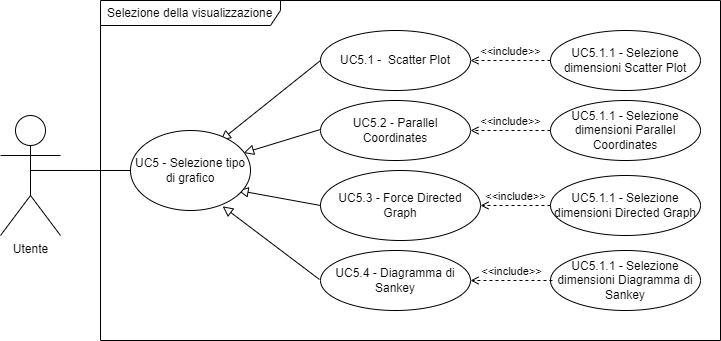
\includegraphics[width=\textwidth]{uc5.png}
 \caption{UC5 - Selezione tipo di grafico}
\end{figure}

 \begin{itemize}
     \item \textbf{Descrizione:} l'utente visualizza varie tipologie di grafico e ne sceglie una;
     \item \textbf{Attore primario:} utente;
     \item \textbf{Precondizioni:} il sistema è stato inizializzato [UC1];
     \item \textbf{Postcondizioni:} viene visualizzato il grafico desiderato;
     \item \textbf{Scenario principale:}
     \begin{enumerate}
       \item L'utente sceglie la visualizzazione desiderata tra quelle disponibili;
     \end{enumerate}
     \item \textbf{Generalizzazioni:} l'utente può selezionare una tra le possibili opzioni:
     \begin{enumerate}
         \item \textit{Scatter Plot} [UC5.1];
         \item \textit{Parallel Coordinates} [UC5.2];
         \item \textit{Force-Directed Graph} [UC5.3];
         \item \textit{Sankey Diagram} [UC5.4].
     \end{enumerate}
 \end{itemize}

\subsection{UC5.1 - Selezione Scatter Plot}
\begin{itemize}
    \item \textbf{Descrizione:} l'utente decide che visualizzazione di \textit{Scatter Plot} vuole vedere;
    \item \textbf{Attore primario:} utente;
    \item \textbf{Precondizioni:} il sistema è stato inizializzato [UC1];
    \item \textbf{Postcondizioni:} viene visualizzato il grafico \textit{Scatter Plot} selezionato;
    \item \textbf{Scenario principale:}
    \begin{enumerate}
      \item L'utente sceglie la visualizzazione desiderata tra quelle disponibili, decidendo tra varie visualizzazioni dello stesso grafico.
    \end{enumerate}
\end{itemize}

\subsection{UC5.2 - Selezione Parallel Coordinates}
\begin{itemize}
    \item \textbf{Descrizione:} l'utente decide che visualizzazione di \textit{Parallel Coordinates} vuole vedere;
    \item \textbf{Attore primario:} utente;
    \item \textbf{Precondizioni:} il sistema è stato inizializzato [UC1];
    \item \textbf{Postcondizioni:} viene visualizzato il grafico \textit{Parallel Coordinates} selezionato;
    \item \textbf{Scenario principale:}
    \begin{enumerate}
    \item L'utente sceglie la visualizzazione desiderata tra quelle disponibili, decidendo tra varie visualizzazioni dello stesso grafico.
    \end{enumerate}
\end{itemize}

\subsection{UC5.3 - Selezione Force-Directed Graph}
\begin{itemize}
    \item \textbf{Descrizione:} l'utente decide che visualizzazione di \textit{Force-Directed Graph} vuole vedere;
    \item \textbf{Attore primario:} utente;
    \item \textbf{Precondizioni:} il sistema è stato inizializzato [UC1];
    \item \textbf{Postcondizioni:} viene visualizzato il grafico \textit{Force-Directed Graph} selezionato;
    \item \textbf{Scenario principale:}
    \begin{enumerate}
      \item L'utente sceglie la visualizzazione desiderata tra quelle disponibili, decidendo tra varie visualizzazioni dello stesso grafico.
    \end{enumerate}
\end{itemize}

\subsection{UC5.4 - Selezione Sankey Diagram}
\begin{itemize}
    \item \textbf{Descrizione:} l'utente decide che visualizzazione di \textit{Sankey Diagram} vuole vedere;
    \item \textbf{Attore primario:} utente;
    \item \textbf{Precondizioni:} il sistema è stato inizializzato [UC1];
    \item \textbf{Postcondizioni:} viene visualizzato il grafico \textit{Sankey Diagram} selezionato;
    \item \textbf{Scenario principale:}
    \begin{enumerate}
      \item L'utente sceglie la visualizzazione desiderata tra quelle disponibili, decidendo tra varie visualizzazioni dello stesso grafico.
    \end{enumerate}
\end{itemize}


\section{UC? - Personalizzazione visualizzazione scelta}
\begin{figure}[H]
  \centering
  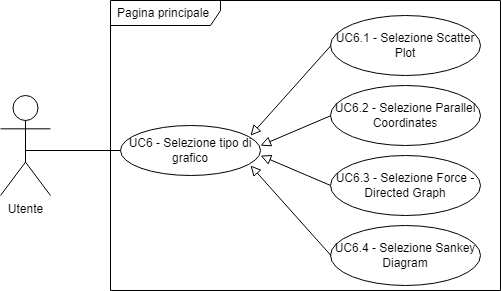
\includegraphics[width=\textwidth]{uc6.png}
  \caption{UC? - Personalizzazione visualizzazione}
\end{figure}

\begin{itemize}
  \item \textbf{Descrizione}: l'utente ha la possibilità di modificare vari aspetti del grafico;
  \item \textbf{Attore primario}: utente;
  \item \textbf{Precondizioni}: l'utente ha selezionato la tipologia di grafico [UC5] e l'applicativo lo ha generato;
  \item \textbf{Postcondizioni}: le modifiche apportate al grafico vengono visualizzate;
  \item \textbf{Scenario principale}:
   \begin{enumerate}
    \item L'utente può impostare varie opzioni del grafico scelto;
    \item Le opzioni scelte vengono visualizzate;
  \end{enumerate}
  \item \textbf{Generalizzazioni}:
    \begin{enumerate}
      \item Personalizzazione \textit{Scatter Plot} [UC?.1];
      \item Personalizzazione \textit{Parallel Coordinates} [UC?.2];
      \item Personalizzazione \textit{Force-Directed Graph} [UC?.3];
      \item Personalizzazione \textit{Sankey Diagram} [UC?.4].
    \end{enumerate}
\end{itemize}

\subsection{UC?.1 - Personalizzazione Scatter Plot}
\begin{figure}[H]
  \centering
  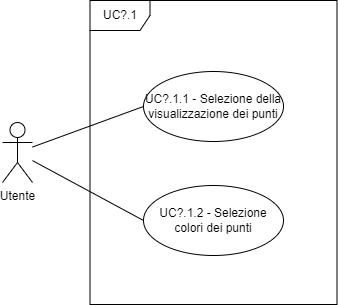
\includegraphics[width=\textwidth]{uc.1.png}
  \caption{UC?.1 - Personalizzazione Scatter Plot}
\end{figure}
\begin{itemize}
    \item \textbf{Descrizione:} l'utente ha la possibilità di modificare vari aspetti del grafico;
    \item \textbf{Attore primario:} utente;
    \item \textbf{Precondizioni:} l’utente ha scelto il grafico \textit{Scatter Plot} [UC5.1];
    \item \textbf{Postcondizioni:} il grafico viene aggiornato;
    \item \textbf{Scenario principale:}
    \begin{enumerate}
      \item L'utente può decidere di:
    \begin{enumerate}
      \item Selezione visualizzazione dei punti [UC?.1.1];
      \item Selezione colori dei punti  [UC?.1.2];
    \end{enumerate}
    \item Le modifiche scelte vengono visualizzate.
  \end{enumerate}
  \end{itemize}

  \subsubsection{UC?.1.1 - Selezione visualizzazione dei punti}
  \begin{itemize}
    \item \textbf{Descrizione:} l'utente ha la possibilità di modificare la forma e la dimensione dei punti;
    \item \textbf{Attore primario:} utente;
    \item \textbf{Precondizioni:} l’utente ha scelto il grafico Scatter Plot [UC5.1];
    \item \textbf{Postcondizioni:} il grafico viene aggiornato;
    \item \textbf{Scenario principale:}
     \begin{enumerate}
      \item L'utente sceglie la forma e la dimensione;
      \item La modifica viene applicata al grafico.
    \end{enumerate}
  \end{itemize}

  \subsubsection{UC?.1.2 - Selezione colori dei punti}
  \begin{itemize}
    \item \textbf{Descrizione:} l'utente ha la possibilità di scegliere i colori dei punti;
    \item \textbf{Attore primario:} utente;
    \item \textbf{Precondizioni:} l’utente ha scelto il grafico Scatter Plot [UC5.1];
    \item \textbf{Postcondizioni:} il grafico viene aggiornato;
    \item \textbf{Scenario principale:}
      \begin{enumerate}
      \item L'utente sceglie i colori;
      \item La modifica viene applicata al grafico.
    \end{enumerate}
  \end{itemize}

\subsection{UC?.2 - Personalizzazione Parallel Coordinates}
\begin{itemize}
    \item \textbf{Descrizione:} l'utente ha la possibilità di modificare vari aspetti del grafico;
    \item \textbf{Attore primario:} utente;
    \item \textbf{Precondizioni:} l’utente ha scelto il grafico \textit{Parallel Coordinates} [UC5.2];
    \item \textbf{Postcondizioni:} le modifiche apportate al grafico vengono visualizzate;
    \item \textbf{Scenario principale:}
    \begin{enumerate}
      \item L'utente ha a disposizione tre slider che permettono di:
    \begin{enumerate}
      \item Cambiare l'opacità del grafico;
      \item Cambiare la curvatura delle linee;
      \item Cambiare la forza di raggruppamento delle linee;
    \end{enumerate}
    \item Il grafico viene modificato in base alla posizione degli slider.
  \end{enumerate}
  \end{itemize}


\subsection{UC?.3 - Personalizzazione Force-Directed Graph}
\begin{figure}[H]
  \centering
  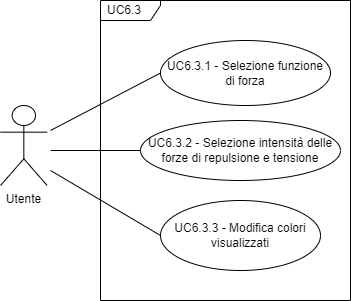
\includegraphics[width=\textwidth]{uc6.3.png}
  \caption{UC?.3 - Personalizzazione Force-Directed Graph}
\end{figure}
\begin{itemize}
    \item \textbf{Descrizione:} l'utente ha la possibilità di modificare vari aspetti del grafico;
    \item \textbf{Attore primario:} utente;
    \item \textbf{Precondizioni:} l’utente ha scelto il grafico \textit{Force-Directed Graph} [UC5.3];
    \item \textbf{Postcondizioni:} il grafico viene aggiornato;
    \item \textbf{Scenario principale:}
    \begin{enumerate}
      \item L'utente può decidere di:
    \begin{enumerate}
      \item Selezionare la funzione di forza [UC?.3.1];
      \item Selezionare l'intensità delle forze di repulsione e tensione [UC?.3.2];
      \item Modificare i colori visualizzati [UC?.3.3];
    \end{enumerate}
    \item Le modifiche scelte vengono visualizzate.
  \end{enumerate}
  \end{itemize}

  \subsubsection{UC?.3.1 - Selezione funzione di forza}
  \begin{itemize}
    \item \textbf{Descrizione:} l'utente ha la possibilità di scegliere quale funzione di forza adottare;
    \item \textbf{Attore primario:} utente;
    \item \textbf{Precondizioni:} l’utente ha scelto il grafico Force-Directed Graph [UC5.3];
    \item \textbf{Postcondizioni:} il grafico viene aggiornato;
    \item \textbf{Scenario principale:}
     \begin{enumerate}
      \item L'utente sceglie la funzione di forza;
      \item La modifica viene applicata al grafico.
    \end{enumerate}
  \end{itemize}

  \subsubsection{UC?.3.2 - Selezione intensità delle forze di repulsione e tensione}
  \begin{itemize}
    \item \textbf{Descrizione:} l'utente ha la possibilità di scegliere quale intensità delle forze attrattive e di tensione adottare;
    \item \textbf{Attore primario:} utente;
    \item \textbf{Precondizioni:} l’utente ha scelto il grafico Force-Directed Graph [UC5.3];
    \item \textbf{Postcondizioni:} il grafico viene aggiornato;
    \item \textbf{Scenario principale:}
      \begin{enumerate}
      \item L'utente sceglie l'intensità delle forze;
      \item La modifica viene applicata al grafico.
    \end{enumerate}
  \end{itemize}

  \subsubsection{UC?.3.3 - Modifica colori visualizzati}
  \begin{itemize}
    \item \textbf{Descrizione:} l'utente ha la possibilità di scegliere quali colori adottare;
    \item \textbf{Attore primario:} utente;
    \item \textbf{Precondizioni:} l’utente ha scelto il grafico Force-Directed Graph [UC5.3];
    \item \textbf{Postcondizioni:} il grafico viene aggiornato;
    \item \textbf{Scenario principale:}
     \begin{enumerate}
      \item L'utente sceglie quali colori associare alle varie dimensioni;
      \item La modifica viene applicata al grafico.
    \end{enumerate}
  \end{itemize}


\subsection{UC?.4 - Personalizzazione Sankey Diagram}
\begin{figure}[H]
  \centering
  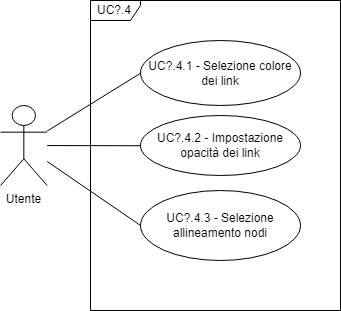
\includegraphics[width=\textwidth]{ucSankey.png}
  \caption{UC?.4 - Personalizzazione Sankey Diagram}
\end{figure}
\begin{itemize}
    \item \textbf{Descrizione:} l'utente ha la possibilità di modificare vari aspetti del grafico;
    \item \textbf{Attore primario:} utente;
    \item \textbf{Precondizioni:} l’utente ha scelto il grafico \textit{Sankey Diagram} [UC5.3];
    \item \textbf{Postcondizioni:} il grafico viene aggiornato;
    \item \textbf{Scenario principale:}
    \begin{enumerate}
      \item L'utente può decidere di:
    \begin{enumerate}
      \item Selezionare il colore dei link [UC?.4.1];
      \item Impostare l'opacità dei link [UC?.4.2];
      \item Selezionare l'allinamento dei nodi [UC?.4.3];
    \end{enumerate}
    \item Le modifiche scelte vengono visualizzate.
  \end{enumerate}
  \end{itemize}

  \subsubsection{UC?.4.1 - Selezione colore dei link}
  \begin{itemize}
    \item \textbf{Descrizione:} l'utente ha la possibilità di scegliere la colorazione dei link, cioè i collegamento tra i nodi;
    \item \textbf{Attore primario:} utente;
    \item \textbf{Precondizioni:} l’utente ha scelto il grafico Sankey Diagram [UC?.4];
    \item \textbf{Postcondizioni:} il grafico viene aggiornato;
    \item \textbf{Scenario principale:}
     \begin{enumerate}
      \item L'utente sceglie la colorazione dei link;
      \item La modifica viene applicata al grafico.
    \end{enumerate}
  \end{itemize}

  \subsubsection{UC?.4.2 - Impostazione opacità dei link}
  \begin{itemize}
    \item \textbf{Descrizione:} l'utente ha la possibilità di impostare l'opacità dei link;
    \item \textbf{Attore primario:} utente;
    \item \textbf{Precondizioni:} l’utente ha scelto il grafico Sankey Diagram [UC?.4];
    \item \textbf{Postcondizioni:} il grafico viene aggiornato;
    \item \textbf{Scenario principale:}
      \begin{enumerate}
      \item L'utente imposta l'opacità dei link;
      \item La modifica viene applicata al grafico.
    \end{enumerate}
  \end{itemize}

  \subsubsection{UC?.4.3 - Selezionare allinamento nodi}
  \begin{itemize}
    \item \textbf{Descrizione:} l'utente ha la possibilità di scegliere l'allineamento dei nodi;
    \item \textbf{Attore primario:} utente;
    \item \textbf{Precondizioni:} l’utente ha scelto il grafico Sankey Diagram [UC?.4];
    \item \textbf{Postcondizioni:} il grafico viene aggiornato;
    \item \textbf{Scenario principale:}
     \begin{enumerate}
      \item L'utente sceglie l'allinamento dei nodi;
      \item La modifica viene applicata al grafico.
    \end{enumerate}
  \end{itemize}

\section{UC7 - Visualizzazione errore scelta filtri}
\begin{itemize}
  \item \textbf{Descrizione}: l'utente imposta dei filtri non validi, quindi visualizza un messaggio di errore esplicativo;
  \item \textbf{Attore primario}: utente;
  \item \textbf{Precondizioni}: l'utente imposta dei filtri che non permettono una corretta visualizzazione del grafico;
  \item \textbf{Postcondizioni}: l'utente visualizza un messaggio di errore e i filtri non vengono applicati;
  \item \textbf{Scenario principale}:
    \begin{enumerate}
      \item L'utente visualizza un messaggio di errore esplicativo.
    \end{enumerate}
\end{itemize}

\section{UC8 - Accesso al manuale utente}
\begin{itemize}
  \item \textbf{Descrizione}: l'utente che ha un dubbio o vuole più informazioni sull'utilizzo dell'applicazione, deve avere accesso rapido al manuale utente;
  \item \textbf{Attore primario}: utente;
  \item \textbf{Precondizioni}: nessuna, l'opzione di accesso ai manuali deve essere sempre disponibile all'utente;
  \item \textbf{Postcondizioni}: viene visualizzato il manuale utente;
  \item \textbf{Scenario principale}:
  \begin{enumerate}
    \item L'utente seleziona il manuale utente;
    \item Viene visualizzato il manuale utente.
  \end{enumerate}
\end{itemize}

\section{UC9 - Salvataggio sessione}
\begin{itemize}
  \item \textbf{Descrizione:} l'utente salva la sessione di lavoro;
  \item \textbf{Attore primario:} utente;
  \item \textbf{Precondizioni:} l'utente ha svolto una sessione di lavoro sull'applicazione, in particolare potrebbe aver scelto un grafico specifico e modificato i parametri personalizzando la visualizzazione;
  \item \textbf{Postcondizioni:} l'utente possiede un file JSON in grado di recuperare grafico e parametri impostati durante la sessione di lavoro;
  \item \textbf{Scenario principale:}
  \begin{enumerate}
    \item L'utente sta lavorando sull'applicazione;
    \item L'utente seleziona la funzionalità ``Salvataggio sessione'';
    \item L'utente salva la sessione corrente.
  \end{enumerate}
\end{itemize}
